\section{Overview} \label{sec:tern-overview}

Multithreaded programs are difficult to write, test, and debug.  A key
reason is nondeterminism: different runs of a multithreaded
program may show different behaviors, depending on how the threads
interleave~\cite{lee06}.

Two main factors make threads interleave nondeterministically.  The first
is \emph{scheduling}, how the OS and hardware schedule threads.
Scheduling nondeterminism is not essential and can be eliminated without
affecting correctness for most programs.  The second is \emph{input}, what
data (\emph{input data}) arrives at what time (\emph{input timing}).
Input nondeterminism sometimes is essential because major changes in
inputs require different schedules.  However, frequently input
nondeterminism is not essential and the same schedule can be used to
process many different inputs (\S\ref{sec:define-schedule}).  We believe
nonessential nondeterminism should be eliminated in favor of determinism.

\emph{Deterministic multithreading} (\dmt)
systems~\cite{dmp:asplos09,coredet:asplos10,kendo:asplos09} make threads
more deterministic by eliminating scheduling nondeterminism.
Specifically, they constrain a multithreaded program such that it always
uses the same thread schedule for the same input.  By doing so, these
systems make program behaviors repeatable, increase testing confidence,
and ease bug reproduction.

Unfortunately, though existing \dmt systems eliminate scheduling
nondeterminism, they do not reduce input nondeterminism.  In fact, they
may aggravate the effects of input nondeterminism because of their design
limitation: when scheduling the threads to process an input, they consider
only this input and ignore previous similar inputs.  This stateless design
makes schedules over-dependent on inputs, so that a slight change to
inputs may force a program to (ad)venture into a vastly different,
potentially buggy schedule, defeating many benefits of determinism.  We
call this the \emph{instability} problem. 
This problem is confirmed by our results (\S\ref{sec:bug-stable}) from
an existing \dmt system~\cite{coredet:asplos10}.

In fact, even with the same input, existing \dmt systems may still force a
program into different schedules for minor changes in the execution
environment such as processor type and shared library.  Thus,
developers may no longer be able to reproduce bugs by running their
program on the bug-inducing input, because their machine may differ from
the machine where the bug occurred.

This paper presents \tern, a schedule-centric, stateful \dmt system.  It
addresses the instability problem using an idea called \emph{schedule
  memoization} that memoizes past working schedules and reuses them for
future inputs.  Specifically, \tern maintains a cache of past schedules and
the input constraints required to reuse these schedules.  When an input arrives,
\tern checks the input against the memoized constraints for a compatible
schedule.  If it finds one, it simply runs the program while enforcing
this schedule.  Otherwise, it runs the program to memoize a schedule and
the input constraints of this schedule for future reuse.  By reusing
schedules, \tern avoids potential errors in unknown schedules.  This
advantage is illustrated in Figure~\ref{fig:idea}.

A real-world analogy to schedule memoization is the natural tendencies in
humans and animals to follow familiar routes to avoid possible hazards
along unknown routes.  Migrant birds, for example, often migrate along
fixed ``flyways.''  We thus name our system after the Arctic Tern, a bird
species that migrates the farthest among all migrants~\cite{artic-tern-wiki}.  

A second advantage of schedule memoization is that it makes schedules
explicit, providing flexibility in deciding when to memoize certain
schedules.  For instance, \tern allows developers to populate a schedule
cache offline, to avoid the overhead of doing so online.  Moreover,
\tern can check for errors (\eg, races) in schedules and memoize only the
correct ones, thus avoiding the buggy schedules and amortizing the
cost of checking for errors.

To make \tern practical, it must handle server programs which frequently
use threads for performance.  These programs present two challenges for
\tern: (1) they often process client inputs (requests) as they arrive, thus
suffering from input timing nondeterminism, which existing \dmt systems do
not handle and (2) they may run continuously, making their schedules
effectively infinite and too specific to reuse.

\tern addresses these challenges using a simple idea called
\emph{windowing}.  Our insight is that server programs tend to return to the
same quiescent states.
% are done processing a batch of inputs.  Based on this insight,
Thus, \tern splits the continuous request stream of a server into
\emph{windows} and lets the server quiesce in between, so that \tern can
memoize and reuse schedules across windows.  Within a window, it admits
requests only at fixed schedule points, reducing timing nondeterminism.

\begin{figure}[t]
\centering
\includegraphics[width=.5\textwidth]{tern/figures/idea.eps}
\caption{\small{\em Advantage of schedule memoization.}  Each solid shape
  represents an input, and each curved line a schedule.  Schedule
  memoization reuses schedules when possible, avoiding bugs in unknown
  schedules and making program behaviors repeatable across similar
  inputs.}
\label{fig:idea}
\end{figure}%% % background on nondeterminism


We implemented \tern in Linux.  It runs as ``parasitic''
user-space schedulers within the application's address space, overseeing
the decisions of the OS scheduler and synchronization library.  It
memoizes and reuses synchronization orders as schedules to increase
performance and reuse rates. It tracks input constraints using
\klee~\cite{klee:osdi08}, a symbolic execution engine.  Our implementation
is software-only, works with general C/C++ programs using threads, and
requires no kernel modifications and only a few lines of modification to
applications, thus simplifying deployment.

We evaluated \tern on a diverse set of 14 programs, including two server
programs Apache~\cite{apache} and MySQL~\cite{mysql}, a parallel
compression utility \pbzip~\cite{pbzip2}, and 11 scientific programs in
\splash~\cite{splash2}.  Our workload included a Columbia CS web trace and
benchmarks used by Apache and MySQL developers.  Our results show that

\begin{enumerate}

\item \tern is easy to use.  For most programs, we modified only a few
  lines to adapt them to \tern.

\item \tern enforces stability across different inputs.  In particular, it
  reused 100 schedules to process 90.3\% of a 4-day Columbia CS web trace.
  Moreover, while an existing \dmt system~\cite{coredet:asplos10} made
  three bugs inconsistently occur or disappear depending on minor input
  changes, \tern always avoided these bugs.

\item \tern has reasonable overhead.  For nine out of fourteen
  evaluated programs, \tern has negligible overhead or improves
  performance; for the other programs, \tern has up to 39.1\%
  overhead.

\item \tern makes threads deterministic.  For twelve out of fourteen
  evaluated programs, the schedules \tern memoized can be deterministically
  reused barring the assumption discussed in \S\ref{sec:impl}.

\end{enumerate}

Our main conceptual contributions are that we identified the instability
problem in existing \dmt systems and proposed two ideas, schedule
memoization and windowing, to mitigate input nondeterminism.  Our
engineering contributions include the \tern system and its evaluation of
real programs.  To the best of our knowledge, \tern is the first stable
\dmt system, the first to mitigate input timing nondeterminism, and the
first shown to work on programs as large, complex, and nondeterministic as
Apache and MySQL.  \tern demonstrates that \dmt has the potential to be
deployed today.

This paper is organized as follows.  We first present a background
(\S\ref{sec:background}) and an overview of \tern (\S\ref{sec:overview}).
We then describe \tern's interface (\S\ref{sec:annotations}), schedule
memoization for batch programs (\S\ref{sec:batch}), and windowing to
extend \tern to server programs (\S\ref{sec:window}).  We then present 
refinements we made to optimize \tern (\S\ref{sec:impl}).  Lastly, we show
our experimental results (\S\ref{sec:evaluation}), discuss related work
(\S\ref{sec:related}), and conclude (\S\ref{sec:conclusion}).
